\documentclass{beamer}

\usepackage[utf8]{inputenc} 
\usepackage[T1]{fontenc}
\usepackage{lmodern}
\usepackage{graphicx}
\usepackage[french]{babel}
\usepackage{tikz}
\usetikzlibrary{arrows,shapes,positioning}


\frenchbsetup{StandardLists=true}
\usetheme{Singapore}
\setbeamertemplate{navigation symbols}{} 
\author{Julien Deguilhem\and Maïlys Denis\and Sébastien Gautheron\and Johann Mitrail\and Anthony Rossi\and Colin Vidal}
\date{}

\setbeamertemplate{footline}{
\begin{beamercolorbox}[]{section in head/foot}
\begin{center}
\insertframenumber{} / \inserttotalframenumber\hspace*{2ex}
\end{center}
\end{beamercolorbox}
}
 
\begin{document}
 
\title{Projet Thésaurus}
\maketitle


\frame{
\frametitle{Introduction}
\begin{itemize}
\item Organisation du projet
\item Modélisation
\item Implémentation
\end{itemize}
}


\begin{frame}
\frametitle{Organisation du projet}
\begin{itemize}
\item réunions tous les 15 jours
\item contacts réguliers par mail
\item gestion des sources via un dépôt Git
\end{itemize}
\end{frame}


\begin{frame}
\frametitle{Répartition des tâches}
\begin{itemize}
\item Julien : implémentation web
\item Colin : infrastructure, modélisation, implémentation BDD
\item Sébastien : réalisation de diagrammes, aide
\item Anthony : chef de projet, design site web
\item Johann : rapport, aide
\item Maïlys : implémentation web, rapport
\end{itemize}
\end{frame}


\begin{frame}
\frametitle{Modélisation}
\begin{center}
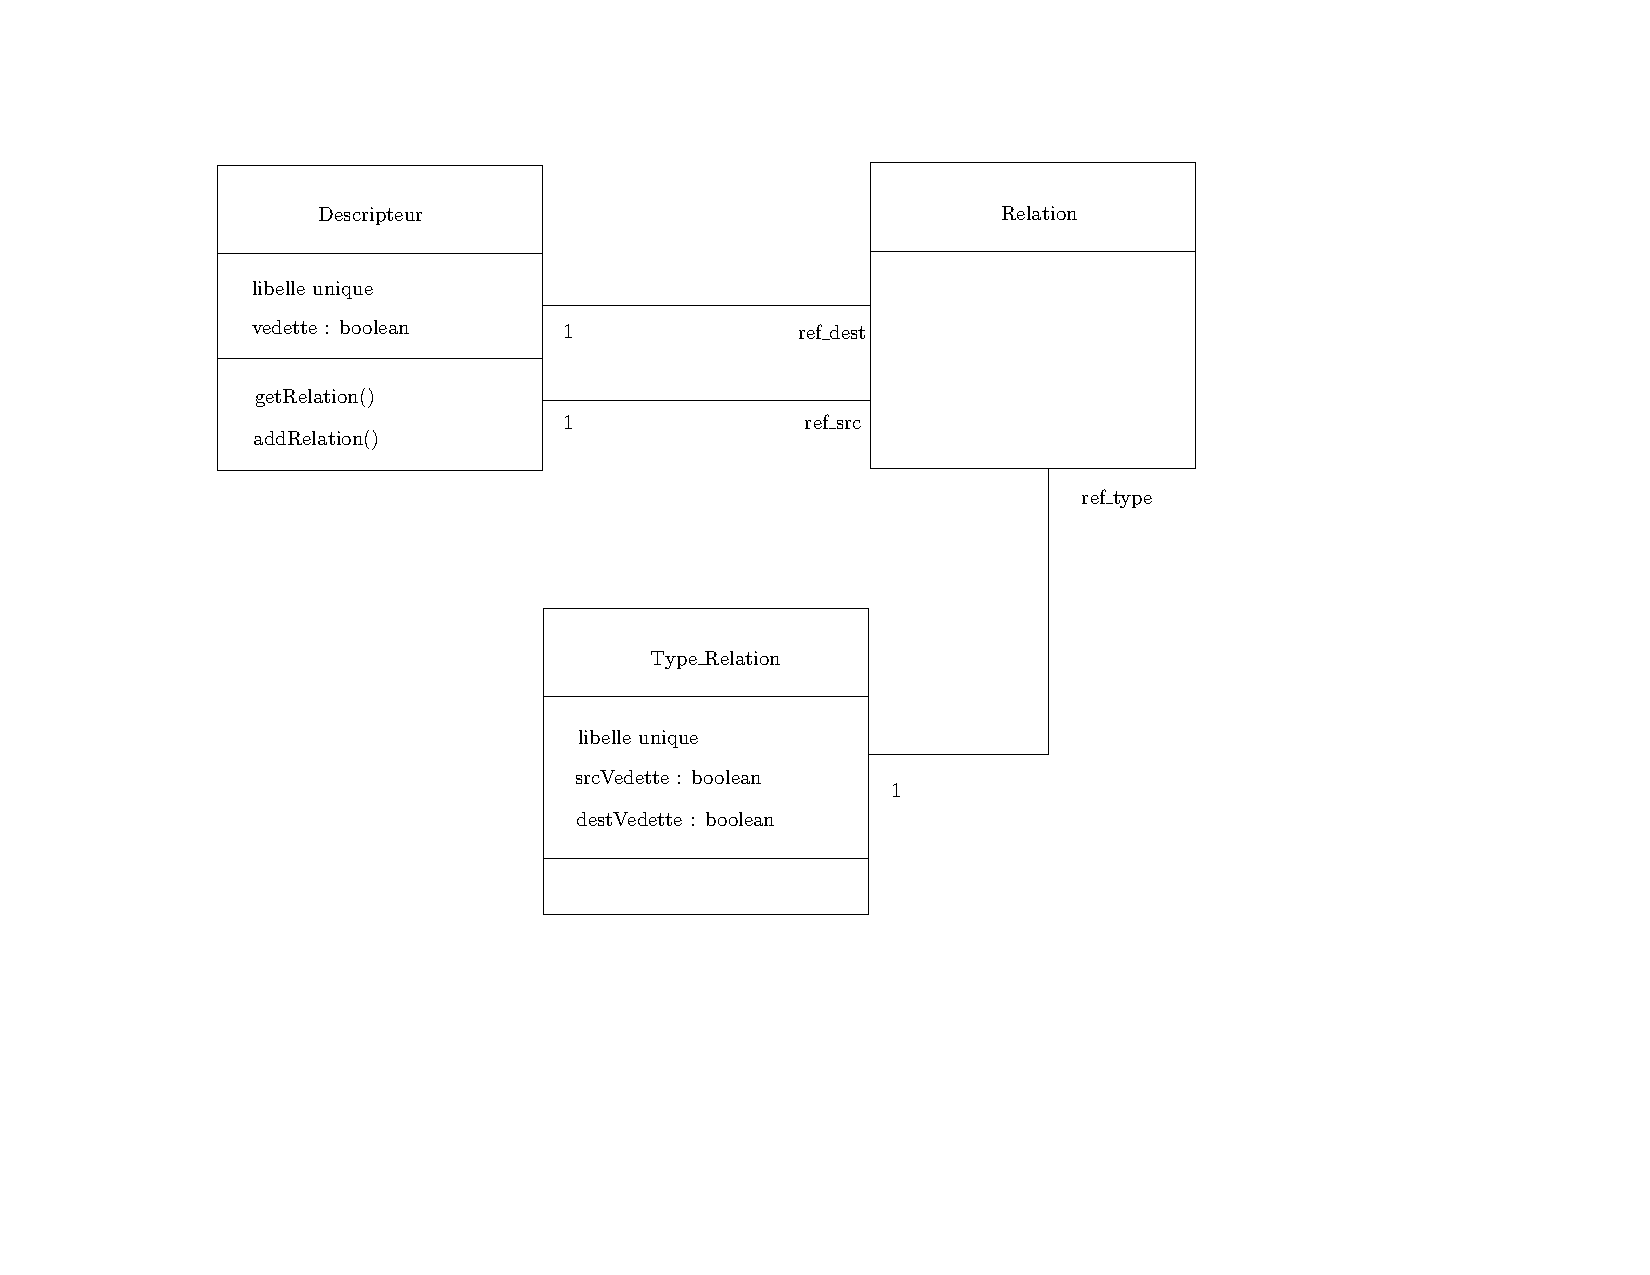
\includegraphics[width=11.5cm, trim = 2cm 1cm 4cm 3cm]{diag_de_classe.pdf}
\end{center}
\end{frame}


\begin{frame}
\frametitle{Modèle sous forme de graphe orienté}
Une relation correspond à un 3-uplet descripteur source, descripteur destination, type relation
\begin{itemize}
\item très généraliste et souple à manipuler
\item déclencheurs pour assurer les contraintes de relations (vedette/non vedette)
\item risque de lenteur sur de gros volumes de données/insertions simultanées multiples
\end{itemize}
\end{frame}


\begin{frame}
\frametitle{Limites conceptuelles}
\begin{itemize}
\item Polysémie
\begin{itemize}
\item \emph{caisse} (= voiture, non vedette)
\item \emph{caisse} (= conteneur, vedette)
\end{itemize}
$\rightarrow$ contrainte d'unicité du couple libellé + état vedette

\item Relations antagonistes
\begin{itemize}
\item \emph{chat} spécialise \emph{félin}
\item \emph{félin} ne généralise PAS \emph{chat}. Le faire est dangereux en cas de polysémie sur le mot \emph{chat} : mettre la relation de généralisation sur \emph{chat (félin)} ou \emph{chat (discussion instantanée)} ?
\end{itemize}
$\rightarrow$ possibilité d'afficher les relations entrantes
\end{itemize}
\end{frame}


\begin{frame}
\frametitle{Infrastructure}
\begin{itemize}
\item Oracle 11g
\item Apache2 + PHP + OCI
\item MV KVM sous CentOS récupérant la dernière version des sources régulièrement
\end{itemize}
\end{frame}



\begin{frame}
\frametitle{Implémentation base de données}
\begin{itemize}
\item Une relation associe deux descripteurs et un type de relation par les références des objets des tables Descripteurs et Type\_Relations (vue objet relationnelle)
\item Déclencheurs (ajout/modification table Relations)
\begin{itemize}
\item unicité 3-uplet réf. desc. source, réf. desc. destination, réf. type relation (impossible d'utiliser les références comme clé primaire)
\item cohérence des associations en fonction du type de relation\\ (ex. relation de type \emph{Synonyme} doit avoir un descripteur source vedette et descripteur destination non vedette)
\end{itemize}
\end{itemize} 
\end{frame}


\begin{frame}
\frametitle{Implémentation web}
\begin{itemize}
\item Classe Descripteur
\begin{itemize}
\item recherche de descripteur / relation
\item ajout de descripteur
\item ajout de relation
\item suppression de relation (non implémenté dans l'interface utilisateur)
\end{itemize}
\item Simplification des URL (module rewrite Apache + htaccess)\\ \emph{domain.tld/index.php?lib=chat} $\rightarrow$ \emph{domain.tld/chat/}
\end{itemize}
\end{frame}


\begin{frame}
\frametitle{Interface utilisateur}
\begin{itemize}
\item design CSS + HTML (Bootstrap)
\item 2 pages principales
\begin{itemize}
\item beuuu
\end{itemize}
\end{itemize}
\end{frame}


\begin{frame}
\frametitle{Conclusion}

\end{frame}

\end{document}
